% Kapitel: Numerische Tests (Element-WENO-M1PN). Stand 12.11.2026.
% Quellen der Zahlen: results/heterogeneous/nx_hetero_20261111/nx_hetero_paper/*.md (nx-Kampagne ew_hetero_paper,
% Git 47b8752), output/line_source_20261110/analysis/REPORT.md (Git 8efe517), docs/ELEMENT_HETEROGENEOUS.md.
% Benötigt: amsmath, booktabs, graphicx, subcaption; Abbildungen in figures/.
\chapter{Numerische Tests}
\label{chap:tests}

In diesem Kapitel definieren wir die numerischen Tests, mit denen das elementbasierte
M1PN-Verfahren mit WENO-stabilisiertem $P_N$-Ziel (im Folgenden \emph{Element-WENO}) geprüft
wird, und stellen die Ergebnisse dar. Die Tests decken drei Fragen ab:
\begin{enumerate}
  \item \textbf{Genauigkeit gegen eine kinetische Referenz.} Der 2D-Lattice-Test besitzt eine
        hochaufgelöste $S_N$-Referenz mit veröffentlichten Kenngrößen \cite{schotthoefer_hauck_2025};
        der Line-Source-Test besitzt eine (gefaltete) analytische Lösung
        \cite{ganapol_2008,garrett_hauck_2013}.
  \item \textbf{Robustheit.} Massenerhaltung, Realisierbarkeit (M1-Kegel) und Stabilität bei
        unstetigen und steifen Materialdaten bis $\sigma_a=10^7$.
  \item \textbf{Effizienz.} Rechenzeit bei gleicher Genauigkeit im Vergleich zu einem unabhängigen
        M1PN-Verfahren mit Massenkorrektur (im Folgenden \emph{Pfad~B}).
\end{enumerate}
Alle gemessenen Abweichungen gegen kinetische Referenzen enthalten den Abbruchfehler des
$P_N$-Winkelmodells. Sie sind deshalb keine reinen Diskretisierungsfehler; Konvergenz in $h$
bedeutet hier Konvergenz gegen die (unbekannte) $P_N$-Lösung, deren Abstand zur kinetischen
Lösung mit $N$ fällt.

\section{Verfahren und Einstellungen}
\label{sec:tests:setup}

Element-WENO verwendet Tensor-Bernstein-Elemente $Q_p$, $p\in\{1,\dots,4\}$, auf uniformen
kartesischen Gittern. Das Hochordnungsziel ist die $P_N$-Galerkin-Diskretisierung mit konsistenter
Masse und der WENO-Stabilisierung nach \cite{kuzmin_hajduk_vedral_2025}; die Momente nullter und
erster Ordnung werden elementweise gegen ein M1-Verfahren niedriger Ordnung mit Bar-States
\cite{moujaes_2025} begrenzt. Absorption, Streuung und Quellen werden knotenweise exakt integriert
und per Strang-Splitting angekoppelt. Zeitintegration ist SSPRK(4,3) mit $\mathrm{CFL}=0.2$.
Mit nicht kommutierender Reaktion ist das Verfahren damit zweiter Ordnung in der Zeit (beobachtet
2.0--2.2); der Zeitfehler liegt bei $\mathrm{CFL}=1$ zwei bis drei Größenordnungen unter dem
Ortsfehler derselben Rechnung (2D-Lattice $Q_1/112$, $P_7$: $8\cdot10^{-5}$ relativ in der Masse gegen
$1.9\,\%$ Ortsfehler), eine höhere Splitting-Ordnung ist daher nicht nötig.
Der WENO-Sensor $1-\gamma_e=r_e^q$ mit $q=1$ ist in $r_e=0$ nicht differenzierbar; an glatten Extrema
auf feinen Gittern koppelt er über die Stabilisierung Rundungsfehler zurück (glatter periodischer
Test: $Q_4$ ab $256$ Elementen Fehler $5\cdot10^{-8}$ statt $10^{-13}$, $Q_1$ und $Q_3$ verlieren
etwas Ordnung). Mit $q=3$ verschwindet der Effekt; wir behalten $q=1$, da er die Tests mit
Unstetigkeiten nicht berührt.
Materialkoeffizienten werden nodal gemittelt,
$\sigma_i=\int\sigma\varphi_i\,dx\big/\int\varphi_i\,dx$.

Pfad~B ist das M1PN-Verfahren mit Massenkorrektur (\texttt{m1pn\_mass\_correction}) auf $Q_1$ mit
gelumpter Masse und SSPRK3. Wir verwenden ihn als unabhängige Vergleichsrechnung.

Die Produktionsläufe der Abschnitte~\ref{sec:tests:lattice}, \ref{sec:tests:lattice3d} und
\ref{sec:tests:shadow} liefen auf dem nx-Cluster (Kampagne \texttt{ew\_hetero\_paper}, eingefrorenes
Binary, 16 Kerne pro Lauf, NUMA-gebunden). Die Line-Source-Läufe
(Abschnitt~\ref{sec:tests:linesource}) stammen aus einer früheren Kampagne mit 16 Threads.

\section{Zweidimensionaler Lattice-Test}
\label{sec:tests:lattice}

\subsection{Definition}

Das Gebiet ist $D=(0,7)^2$, unterteilt in die Einheitszellen
$C_{ij}=[i-1,i]\times[j-1,j]$, $i,j=1,\dots,7$. Die Absorberzellen sind
\[
  \mathcal B=\{C_{22},C_{42},C_{62},C_{33},C_{53},C_{24},C_{64},C_{35},C_{55},C_{26},C_{66}\},
\]
die Quellzelle ist $C_{44}=[3,4]^2$, alle übrigen Zellen sind rein streuend. Die Koeffizienten sind
\begin{center}
\begin{tabular}{lcccc}
  \toprule
  Bereich & $\sigma_t$ & $\sigma_s$ & $\sigma_a$ & $q$ \\
  \midrule
  Absorber $\mathcal B$ & 10 & 0 & 10 & 0 \\
  Quelle $C_{44}$       & 1  & 1 & 0  & 1 \\
  übrige Zellen         & 1  & 1 & 0  & 0 \\
  \bottomrule
\end{tabular}
\end{center}
bei Teilchengeschwindigkeit eins, isotroper Streuung und isotroper Quelle. Die Endzeit ist $T=3.2$.
Wir verwenden die Anfangsdaten $\psi^{(0)}=10^{-10}$, $\psi^{(l\ge1)}=0$ und Vakuum-Einstrom.
Geometrie und Material stimmen mit \cite{moujaes_2025} (Gl.~(44)--(47)) und
\cite{schotthoefer_hauck_2025} (dort auf $[-3.5,3.5]^2$ verschoben) überein. Abweichungen:
\cite{schotthoefer_hauck_2025} startet mit $\psi_0=0$, \cite{moujaes_2025} verwendet einen
do-nothing-Auslass. Bis $T$ verlassen bei uns nur $5\cdot10^{-7}$ bis $8\cdot10^{-5}$ der
injizierten Masse das Gebiet; für die globalen Kenngrößen ist der Unterschied der Randbehandlung
damit vernachlässigbar.

\paragraph{Kenngrößen.} Mit der Dichte $\rho=\int_{S^2}\psi\,d\Omega$ betrachten wir
\[
  M(T)=\int_D\rho(T)\,dx,\qquad
  A=\int_0^T\!\!\int_{\mathcal B}\sigma_a\rho\,dx\,dt,\qquad
  R(T)=\int_{\mathcal B}\sigma_a\rho(T)\,dx,
\]
also die Masse bei $T$, die Gesamtabsorption und die Absorptionsrate bei $T$. Sie entsprechen
QoI-5, QoI-4 und QoI-3 in \cite[Tab.~1]{schotthoefer_hauck_2025}. Dort ist die Konzentration über
eine Halbkugel integriert; in unseren Einheiten (Faktor $1/(2\pi)$) lauten die Referenzwerte
\[
  M_{\mathrm{ref}}=2.0802,\qquad A_{\mathrm{ref}}=1.1195,\qquad R_{\mathrm{ref}}=0.7316 .
\]
Die Referenz ist der Mittelwert von neun $S_N$-Rechnungen (Tessellationsquadratur bis $4\cdot22^2$
Richtungen, Zellweite bis $h=10^{-3}$); die relative Streuung dieser Rechnungen liegt bei
$5.5\cdot10^{-5}$ ($M$), $5.5\cdot10^{-4}$ ($A$) und $7.3\cdot10^{-5}$ ($R$) und ist damit
gegenüber allen hier gemessenen Abweichungen vernachlässigbar.

\paragraph{Gitter.} $P_N$ mit $N\in\{3,7,11\}$; $Q_1/112$, $Q_2/56$, $Q_3/35$, $Q_4/28$
(je 113 bzw.\ 106 Kontrollpunkte pro Achse) sowie die Verfeinerungen $Q_1/224$ und $Q_2/112$
(225 Punkte). Die Elementzahl ist durch 7 teilbar, die Materialsprünge liegen also auf
Elementkanten.

\subsection{Ergebnisse}

\begin{table}[htbp]
  \centering
  \small
  \begin{tabular}{llrrrrr}
    \toprule
    Verfahren & $P_N$ & $Q_p/E$ & $\Delta M$ & $\Delta A$ & $\Delta R$ & Zeit [s] \\
    \midrule
    Element-WENO & $P_3$    & $Q_1/112$ & $-3.14\,\%$ & $+5.87\,\%$ & $+7.13\,\%$ & 7.5 \\
                 & $P_7$    & $Q_1/112$ & $-1.91\,\%$ & $+3.58\,\%$ & $+2.20\,\%$ & 9.5 \\
                 & $P_7$    & $Q_1/224$ & $-0.87\,\%$ & $+1.65\,\%$ & $+1.28\,\%$ & 60.5 \\
                 & $P_7$    & $Q_2/112$ & $-1.25\,\%$ & $+2.35\,\%$ & $+1.71\,\%$ & 40.4 \\
                 & $P_{11}$ & $Q_1/112$ & $-1.80\,\%$ & $+3.37\,\%$ & $+2.06\,\%$ & 12.2 \\
                 & $P_{11}$ & $Q_1/224$ & $-0.63\,\%$ & $+1.20\,\%$ & $+0.96\,\%$ & 73.9 \\
                 & $P_{11}$ & $Q_2/112$ & $-1.00\,\%$ & $+1.89\,\%$ & $+1.45\,\%$ & 53.3 \\
    \midrule
                 & $P_{11}$ & $Q_2/56$  & $-2.76\,\%$ & $+5.16\,\%$ & $+3.12\,\%$ & 9.0 \\
                 & $P_{11}$ & $Q_3/35$  & $-3.91\,\%$ & $+7.29\,\%$ & $+3.81\,\%$ & 17.9 \\
                 & $P_{11}$ & $Q_4/28$  & $-4.50\,\%$ & $+8.38\,\%$ & $+4.14\,\%$ & 15.8 \\
    \midrule
    Pfad B       & $P_3$    & $Q_1/112$ & $-2.98\,\%$ & --          & $+6.90\,\%$ & 87.8 \\
                 & $P_7$    & $Q_1/112$ & $-1.83\,\%$ & --          & $+2.05\,\%$ & 121.7 \\
    \bottomrule
  \end{tabular}
  \caption{2D-Lattice, relative Abweichung von Masse $M(T)$, Gesamtabsorption $A$ und
           Absorptionsrate $R(T)$ gegen die kinetische Referenz \cite{schotthoefer_hauck_2025}
           sowie Lösezeit (16 Kerne). Pfad~B rechnet mit dem kleineren historischen Zeitschritt
           $\Delta t=5.2\cdot10^{-4}$; Element-WENO mit demselben $\Delta t$ ändert die Kenngrößen um
           weniger als $10^{-4}$ (P7: 57.5\,s). Pfad~B liefert keine Gesamtabsorption.}
  \label{tab:lattice}
\end{table}

\begin{figure}[htbp]
  \centering
  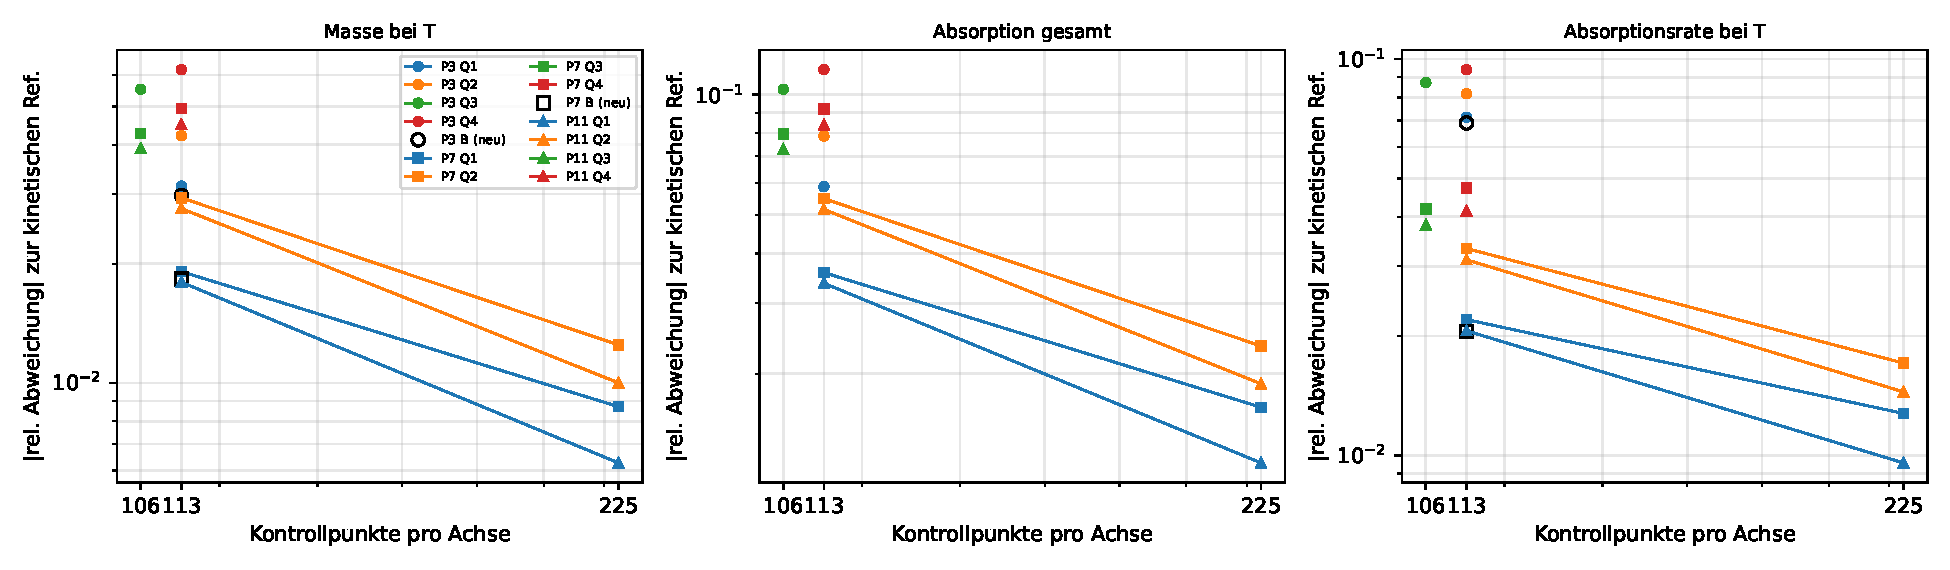
\includegraphics[width=\textwidth]{figures/lattice_convergence.pdf}
  \caption{2D-Lattice: Betrag der relativen Abweichung von $M(T)$, $A$ und $R(T)$ zur kinetischen
           Referenz über der Zahl der Kontrollpunkte pro Achse. Linien verbinden Läufe gleichen
           Grads; offene Symbole sind Pfad~B.}
  \label{fig:lattice:conv}
\end{figure}

\begin{figure}[htbp]
  \centering
  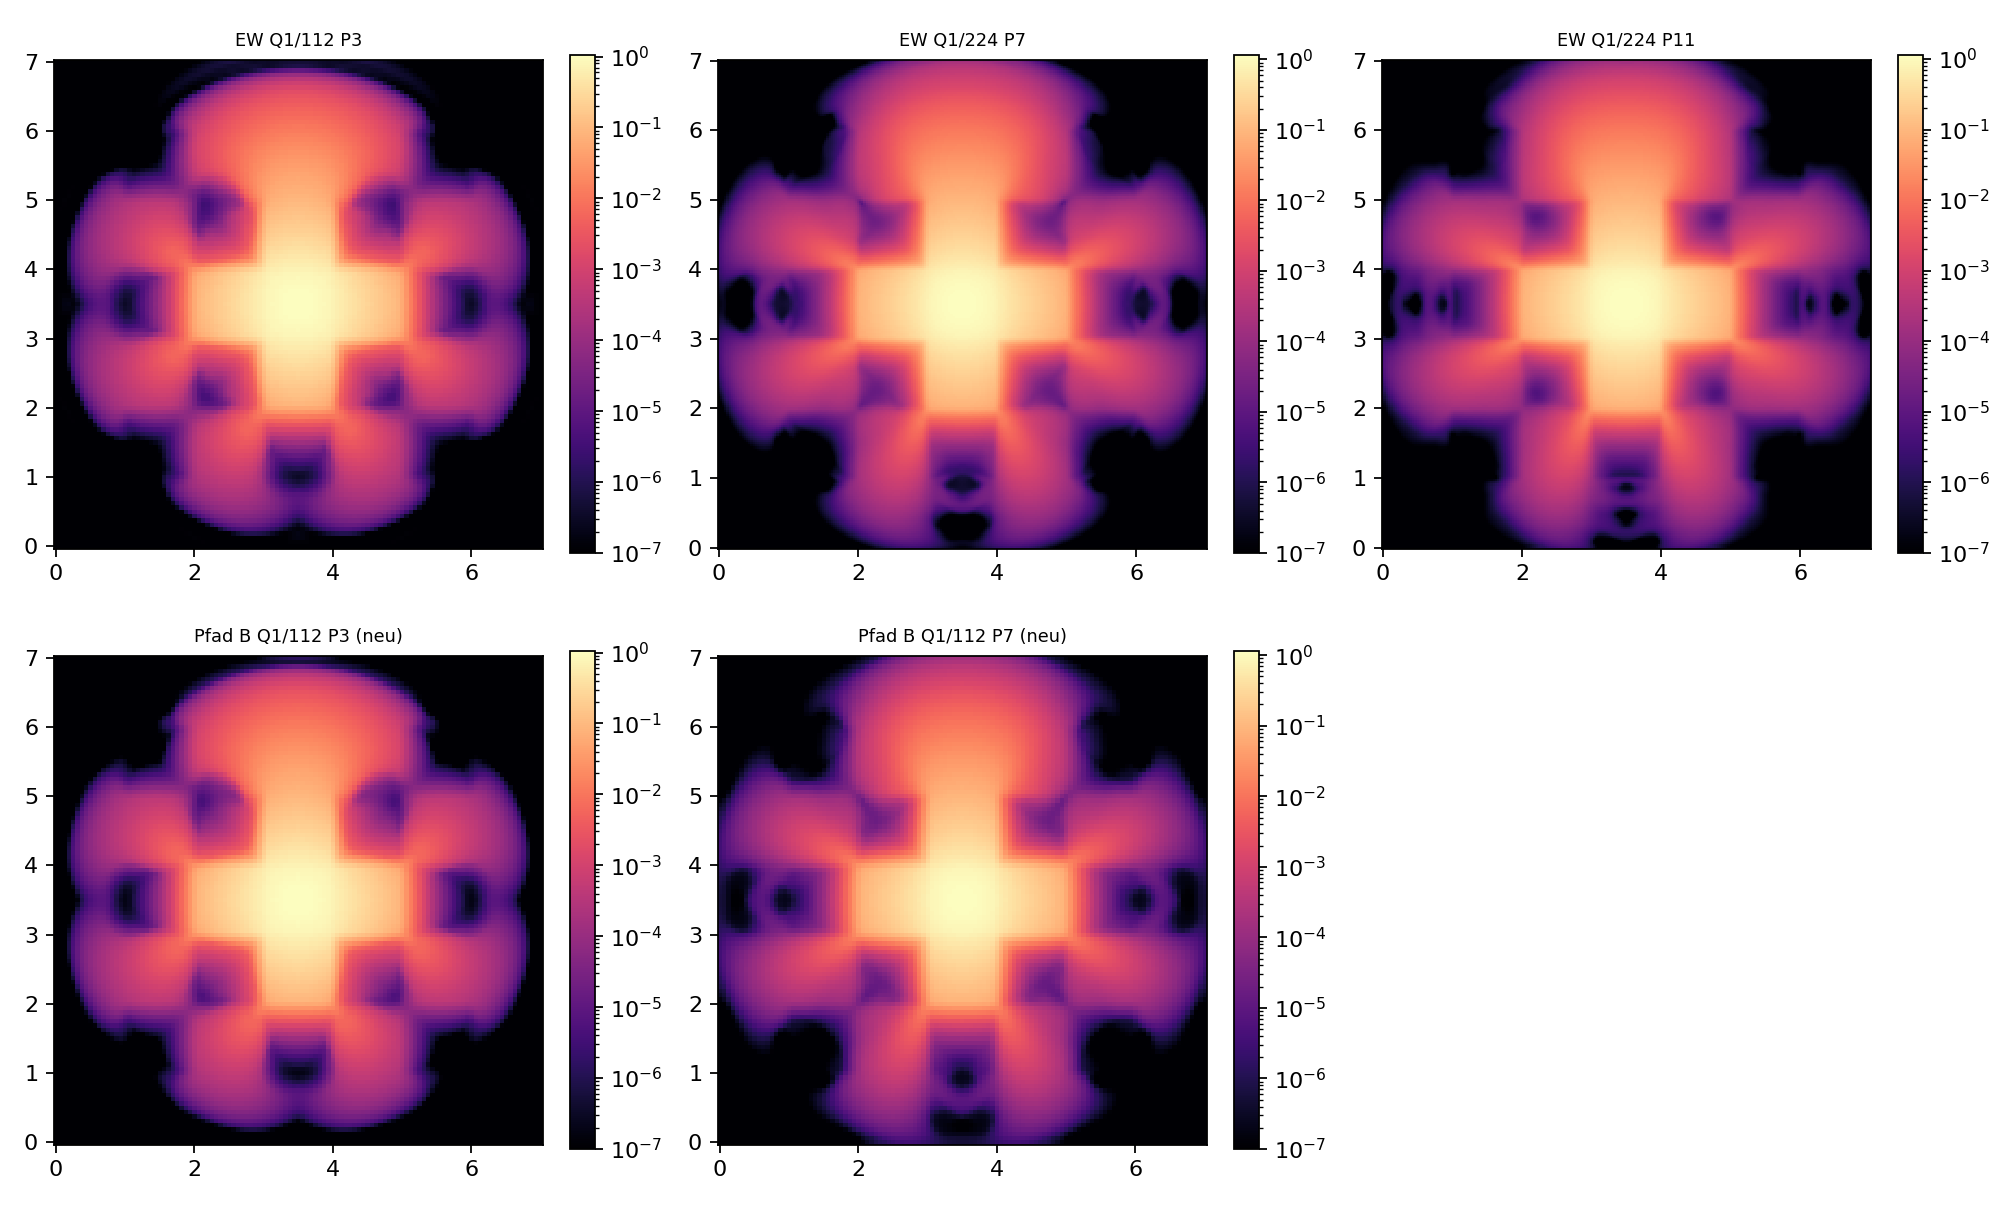
\includegraphics[width=\textwidth]{figures/lattice_density_maps.png}
  \caption{2D-Lattice: Dichte $\rho(T)$ (logarithmisch, $10^{-7}$ bis $1$). Oben Element-WENO
           ($P_3$ auf $Q_1/112$, $P_7$ und $P_{11}$ auf $Q_1/224$), unten Pfad~B auf $Q_1/112$.}
  \label{fig:lattice:maps}
\end{figure}

\paragraph{Konvergenz in $h$.} Bei Verdopplung der Auflösung von 113 auf 225 Punkte pro Achse
fallen alle drei Abweichungen um den Faktor 2 bis 3 (Tabelle~\ref{tab:lattice},
Abbildung~\ref{fig:lattice:conv}). Für $P_{11}$ auf $Q_1/224$ bleiben $-0.6\,\%$ in der Masse und
$+1.0\,\%$ in der Absorptionsrate. Der verbleibende Fehler ist damit räumlich dominiert. Der
Zeitfehler ist vernachlässigbar: Ein 6.5-mal kleinerer Zeitschritt ändert die Kenngrößen um weniger
als $10^{-4}$.

\paragraph{Konvergenz in $N$.} Von $P_3$ nach $P_7$ halbieren sich die Abweichungen etwa; von
$P_7$ nach $P_{11}$ ist der Gewinn klein. Auf den untersuchten Gittern ist ab $N=7$ also der
Ortsfehler bestimmend.

\paragraph{Polynomgrad bei gleicher Punktzahl.} Bei gleicher Zahl an Kontrollpunkten nimmt die
Genauigkeit mit steigendem Grad ab: $Q_1>Q_2>Q_3>Q_4$ (für $P_{11}$: $\Delta M$ von $-1.8\,\%$
auf $-4.5\,\%$). Die Lösung besitzt an den Materialsprüngen nur geringe Regularität; die nodale
Mittelung des Materials ist von erster Ordnung, und größere Elemente verschmieren die Sprünge über
eine größere Breite. Für heterogene Probleme dieses Typs sind deshalb niedrige Grade auf feinen
Gittern vorzuziehen.

\paragraph{Vergleich mit Pfad~B.} Auf demselben Gitter $Q_1/112$ stimmen beide Verfahren bis auf
etwa $0.2$ Prozentpunkte überein ($P_7$: $\Delta M=-1.91\,\%$ gegen $-1.83\,\%$). Element-WENO
benötigt dafür 9.5\,s statt 122\,s, also etwa ein Zwölftel der Rechenzeit; bei gleichem
Zeitschritt ist es immer noch etwa doppelt so schnell. Die Dichtekarten
(Abbildung~\ref{fig:lattice:maps}) zeigen dieselben Strukturen.

\paragraph{Wellenstrukturen hinter den Absorbern.} Hinter den drei Absorberblöcken auf den Achsen
durch die Quelle ($C_{24}$, $C_{64}$, $C_{42}$) zeigen die Karten bei $P_7$ und $P_{11}$
Keulen bei Dichten zwischen $10^{-8}$ und $10^{-5}$. Ihre Zahl hängt von $N$ ab (auf der Linie
$y=3.5$ zwei Minima bei $P_7$, drei bei $P_{11}$), ihre Lage kaum vom Gitter (Minima bei $P_{11}$:
$x=0.38/0.44/0.47$ für $Q_1/112$, $Q_2/112$, $Q_1/224$), und Pfad~B zeigt dasselbe Muster. Es
handelt sich um die Überlagerung der $(N+1)/2$ Wellenfronten des $P_N$-Systems im nahezu leeren
Schattengebiet, also um eine Eigenschaft des Modells, nicht des Verfahrens. Für die Kenngrößen sind
sie ohne Bedeutung.

\subsection{Einordnung in die Literatur}

Für den Lattice-Test gibt es mit \cite{schotthoefer_hauck_2025} erstmals eine Referenz, gegen die
andere Arbeiten Fehler in denselben Kenngrößen angeben. Tabelle~\ref{tab:lattice:lit} stellt die
Absorptionsrate $R(T)$ (QoI-3) zusammen.

\begin{table}[htbp]
  \centering
  \small
  \begin{tabular}{p{6.2cm}p{4.2cm}r}
    \toprule
    Verfahren & Quelle & $|\Delta R|$ \\
    \midrule
    Streuung der neun $S_N$-Referenzrechnungen & \cite{schotthoefer_hauck_2025} & $0.007\,\%$ \\
    $S_N$ (KiT-RT), niedrig aufgelöst          & \cite{gonzales_2026}           & $6.60\,\%$ \\
    Neuronales Surrogat (Transolver)          & \cite{gonzales_2026}           & $1.06\,\%$ \\
    Neuronales Surrogat (BSMS-MGN)            & \cite{gonzales_2026}           & $0.28\,\%$ \\
    \midrule
    Pfad~B, $P_7$, $Q_1/112$                  & diese Arbeit & $2.05\,\%$ \\
    Element-WENO, $P_3$, $Q_1/112$            & diese Arbeit & $7.13\,\%$ \\
    Element-WENO, $P_7$, $Q_1/224$            & diese Arbeit & $1.28\,\%$ \\
    Element-WENO, $P_{11}$, $Q_1/224$         & diese Arbeit & $0.96\,\%$ \\
    \bottomrule
  \end{tabular}
  \caption{Relative Abweichung der Absorptionsrate bei $T=3.2$ (QoI-3) gegen die kinetische
           Referenz. Die Surrogate in \cite{gonzales_2026} sind auf hochaufgelöste $S_N$-Daten
           trainiert; sie lösen kein Transportmodell, sondern approximieren die Referenzlösung.
           Unsere Werte enthalten den $P_N$-Abbruchfehler.}
  \label{tab:lattice:lit}
\end{table}

Zur Kontrolle der Referenz selbst haben wir eine eigene Monte-Carlo-Rechnung durchgeführt
(Transport mit Geschwindigkeit 1, exakte Zellgeometrie, implizites Einfangen, $4\cdot10^{10}$
Historien, statistischer Fehler $\approx10^{-5}$ relativ; validiert am ungestoßenen Anteil gegen
dessen Strahlintegral). Sie ergibt $M(T)=2.080890$, $A=1.119098$ und $R(T)=0.731555$ (in
Einheiten von $\rho$, also Tabelle~1 aus \cite{schotthoefer_hauck_2025} geteilt durch $2\pi$). Die
Literaturwerte weichen davon um $-0.033\,\%$, $+0.036\,\%$ und $+0.006\,\%$ ab, also innerhalb ihrer
vier Stellen. Die Abweichungen in Tabelle~\ref{tab:lattice} verschieben sich gegen Monte Carlo
entsprechend um höchstens $0.04$ Prozentpunkte; die Aussagen bleiben unverändert.
Mit der Referenz lassen sich auch feinere Rechnungen bewerten: Mit First-Collision-Source liegen
$P_{35}$ auf $896^2$ Elementen bei $-0.044\,\%$, $+0.075\,\%$ und $+0.074\,\%$ (Masse, Absorption,
Rate); ab $896^2$ ändert die Gitterverfeinerung wenig, der verbleibende Fehler ist überwiegend
$P_N$-Fehler. Gegen die Tabelle aus \cite{schotthoefer_hauck_2025} sähe derselbe Lauf mit
$-0.011\,\%$ in der Masse um den Faktor vier genauer aus.

Ein $P_{11}$-Lauf auf $225^2$ Kontrollpunkten erreicht damit die Genauigkeit eines auf die
Referenz trainierten neuronalen Surrogats und ist deutlich genauer als die niedrig aufgelöste
$S_N$-Rechnung in \cite{gonzales_2026}. Zwei weitere Arbeiten untersuchen verwandte Lattice-Probleme,
sind aber nicht direkt vergleichbar:
\begin{itemize}
  \item \cite{kim_2026} rechnet den \emph{stationären} Lattice mit dem M1-Modell und gibt für die
        Levermore-Schließung einen relativen $L^2$-Fehler der Lösung von $17\,\%$ gegen Monte Carlo
        an (mit gelernter Schließung $7.5\,\%$). Das zeigt, dass M1 allein in diesem Problem einen
        erheblichen Modellfehler besitzt.
  \item \cite{plumridge_2025} vergleicht gefilterte $P_N$-Lösungen ($N\le9$) gegen eine
        $P_{37}$-Lösung auf einer Variante mit der Quelle im Absorber. Der $L^2$-Fehler des
        ungefilterten $P_N$ fällt dort bei $T=3.2$ von $0.027$ ($N=3$) auf $0.007$ ($N=9$). Dies ist
        ein reiner Winkelmodellfehler ohne Bezug zur kinetischen Lösung.
\end{itemize}

\section{Line Source}
\label{sec:tests:linesource}

\subsection{Definition}

Der Line-Source-Test \cite{garrett_hauck_2013} beschreibt einen isotropen Puls entlang einer
unendlichen Linie in einem homogenen Medium. In der Ebene senkrecht zur Linie gilt
\[
  \partial_t\psi+\Omega\cdot\nabla\psi+\sigma_t\psi=\frac{\sigma_s}{4\pi}\int_{S^2}\psi\,d\Omega',
  \qquad
  \psi(x,\Omega,0)=\frac{1}{4\pi}\max\Bigl(\frac{1}{2\pi\varsigma^2}e^{-|x|^2/(2\varsigma^2)},\,
  \rho_{\mathrm{floor}}\Bigr).
\]
Wir verwenden zwei Varianten:
\begin{itemize}
  \item \textbf{GH} (mit Streuung, \cite{garrett_hauck_2013}): $D=[-1.5,1.5]^2$, $\sigma_s=1$,
        $\sigma_a=0$, $T=1$, $\varsigma=0.03$, $\rho_{\mathrm{floor}}=10^{-4}$, Vakuumrand.
        Referenz ist die analytische Lösung \cite{ganapol_2008}, mit dem Gauß-Puls gefaltet
        (Formeln nach \cite{bennett_mcclarren_2022}, Massenkontrolle $10^{-5}$).
        Element-WENO rechnet die exakt auf $[0,1]^2$ skalierte Fassung ($\sigma_s=3$, $T=1/3$,
        $\varsigma=0.01$, Filterstärke $\times3$) und wird auf physikalische Koordinaten
        zurückgerechnet ($r=3r'$, $\rho=\rho'/9$).
  \item \textbf{VOID} (ohne Material): dieselbe Anordnung ohne Streuung auf $[0,1]^2$
        ($T=1/3$, $\varsigma=0.01$). Referenz ist die analytische ungestreute Linienquelle,
        ebenfalls gefaltet.
\end{itemize}
Gemessen wird der relative $L^1$-Fehler der Dichte bei $T$. Gerechnet wurde mit $P_3$, $P_7$,
$P_{11}$, für Pfad~B auf $256^2$ und $512^2$ Zellen, für Element-WENO mit $p=1,\dots,4$ bei gleicher
Knotenzahl, jeweils ohne und mit konstantem Winkelfilter (\enquote{+F}).

\subsection{Ergebnisse}

\begin{table}[htbp]
  \centering
  \small
  \setlength{\tabcolsep}{4pt}
  \begin{tabular}{llrrrrrrrr}
    \toprule
    & & \multicolumn{2}{c}{Pfad B} & \multicolumn{3}{c}{Element-WENO} & \multicolumn{3}{c}{Element-WENO +F} \\
    \cmidrule(lr){3-4}\cmidrule(lr){5-7}\cmidrule(lr){8-10}
    Gitter & $P_N$ & ohne & +F & $p=1$ & $p=2$ & $p=4$ & $p=1$ & $p=2$ & $p=4$ \\
    \midrule
    $256^2$ & $P_3$    & 1.337 & 0.520 & 1.400 & 1.279 & 0.980 & 0.530 & 0.521 & 0.468 \\
            & $P_7$    & 1.013 & 0.118 & 1.045 & 1.008 & 0.823 & 0.130 & 0.137 & 0.142 \\
            & $P_{11}$ & 0.767 & 0.381 & 0.844 & 0.831 & 0.693 & 0.421 & 0.435 & 0.444 \\
    $512^2$ & $P_3$    & 1.333 & 0.544 & 1.443 & 1.444 & 1.185 & 0.545 & 0.544 & 0.531 \\
            & $P_7$    & 1.096 & 0.149 & 1.110 & 1.100 & 1.003 & 0.152 & 0.153 & 0.138 \\
            & $P_{11}$ & 0.927 & 0.432 & 0.943 & 0.936 & 0.860 & 0.442 & 0.446 & 0.467 \\
    \bottomrule
  \end{tabular}
  \caption{Line Source GH: relativer $L^1$-Fehler der Dichte bei $T=1$ gegen die gefaltete
           analytische Lösung. Element-WENO bei gleicher Knotenzahl wie Pfad~B.}
  \label{tab:linesource}
\end{table}

\begin{figure}[htbp]
  \centering
  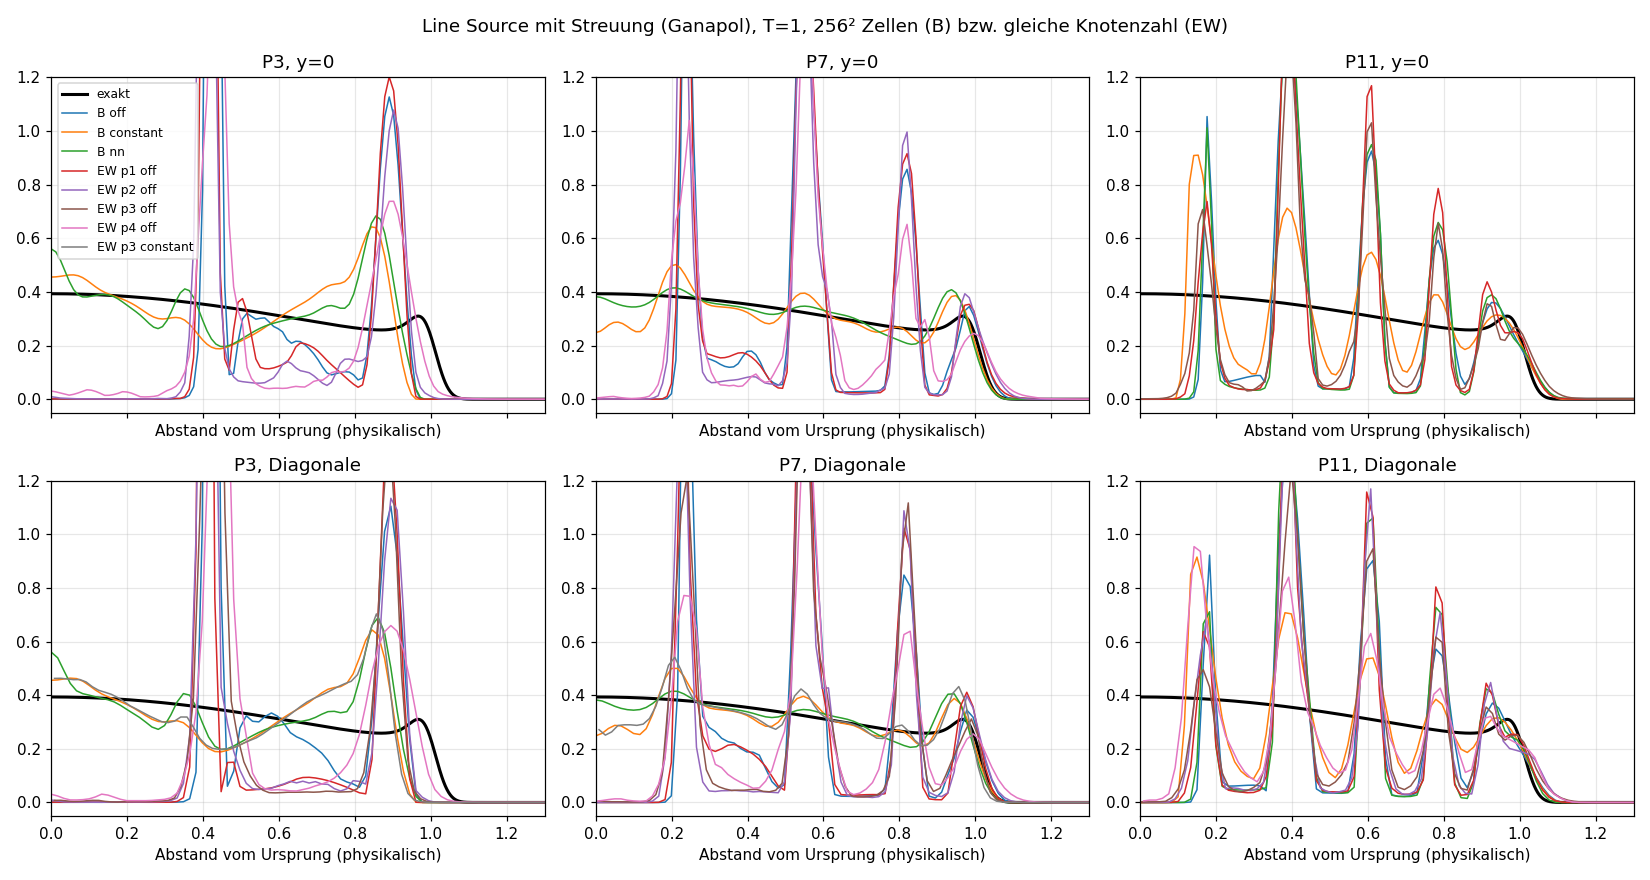
\includegraphics[width=\textwidth]{figures/linesource_GH_g256.png}
  \caption{Line Source GH, $T=1$, $256^2$: Dichteprofile entlang $y=0$ (oben) und der Diagonalen
           (unten) für $P_3$, $P_7$, $P_{11}$ gegen die exakte Lösung (schwarz).}
  \label{fig:linesource}
\end{figure}

\paragraph{Beobachtungen.}
\begin{itemize}
  \item Ohne Filter liegt der relative $L^1$-Fehler aller Verfahren zwischen 0.7 und 1.4
        (Tabelle~\ref{tab:linesource}). Die Lösung besteht aus $N$-abhängigen Ringen
        (Abbildung~\ref{fig:linesource}); das ist das bekannte Verhalten von $P_N$ bei diesem
        Test \cite{garrett_hauck_2013,laiu_2016}. Der Fehler fällt mit der Gitterverfeinerung
        nicht, weil er vom Winkelmodell dominiert wird.
  \item Mit Filter sinkt der Fehler bei $P_7$ auf 0.12--0.15. Element-WENO und Pfad~B liegen
        mit und ohne Filter gleichauf; der Polynomgrad spielt mit Filter kaum eine Rolle.
  \item Bei $P_{11}$ ist der gefilterte Fehler größer als bei $P_7$ (0.38--0.47). Die
        Filterstärke ist für $P_{11}$ also nicht gut gewählt.
  \item In VOID ohne Streuung liegt der Fehler zwischen 0.41 und 0.97; dort nimmt er für
        Element-WENO mit dem Grad ab ($P_{11}$: 0.86 bei $p=1$, 0.43 bei $p=4$).
\end{itemize}

\paragraph{Einordnung.} \cite{garrett_hauck_2013} und \cite{laiu_2016} vergleichen Schließungen am
Line Source qualitativ anhand von Profilen; \cite{laiu_2016} gibt $L^2$-Fehler nur graphisch an.
\cite{plumridge_2025} berichtet für eine Line-Source-Variante mit $T=0.75$ relative Fehler, die für
ungefilterte $P_N$ ($N\le9$) ebenfalls von der Größenordnung eins sind und durch Filter um eine
Größenordnung sinken. Unsere Werte sind damit konsistent. Ein direkter Zahlenvergleich ist wegen
abweichender Endzeit, Glättung und Fehlernorm nicht möglich.

Die Line-Source-Läufe verwenden einen älteren Stand des Verfahrens (Git 8efe517), vor den
Randkorrekturen. Da die Lösung bis $T$ den Rand nicht erreicht, erwarten wir keinen Einfluss;
geprüft ist das nicht.

\section{Dreidimensionaler Lattice-Test}
\label{sec:tests:lattice3d}

\subsection{Definition}

Als eigene Erweiterung ohne Literaturreferenz (Referenz: eigene Monte-Carlo-Rechnung, siehe unten) verwenden wir $D=(0,7)^3$ mit Einheitszellen
$C_{ijk}=[i,i+1]\times[j,j+1]\times[k,k+1]$. Die Absorberzellen sind
\[
  \mathcal A=\bigl\{(i,j,k)\in\{1,\dots,5\}^3:\ i+j+k\ \text{gerade}\bigr\}\setminus\{(4,2,2)\}
  \cup\{(3,3,1)\}\qquad(62\ \text{Zellen}),
\]
mit $\sigma_a=10$ auf $\mathcal A$, sonst $0$; $\sigma_s=0$ auf $\mathcal A$, $\sigma_s=5$ in den
nicht absorbierenden Zellen mit $k=5$ und sonst $\sigma_s=1$; die Quelle $q_0=1$ sitzt in $C_{333}$.
Das Entfernen von $(4,2,2)$ und das Hinzufügen von $(3,3,1)$ brechen alle Spiegelsymmetrien. Der
Test deckt Materialsprünge in allen drei Richtungen, axialen und diagonalen Transport, Schatten und
Mehrfachstreuung ab. $T=3.2$, Vakuum-Einstrom.

\subsection{Ergebnisse}

\begin{table}[htbp]
  \centering
  \small
  \begin{tabular}{llrrrrr}
    \toprule
    $P_N$ & $Q_p/E$ & Punkte & $M(T)$ & $A$ & Bilanz & Zeit [s] \\
    \midrule
    $P_3$ & $Q_2/14$ & 29 & 0.3284 & 2.8715 & $1.9\cdot10^{-13}$ & 12 \\
    $P_3$ & $Q_1/28$ & 29 & 0.4060 & 2.7940 & $1.1\cdot10^{-12}$ & 24 \\
    $P_3$ & $Q_2/28$ & 57 & 0.4917 & 2.7083 & $6.2\cdot10^{-12}$ & 139 \\
    $P_7$ & $Q_2/14$ & 29 & 0.3295 & 2.8703 & $6.2\cdot10^{-13}$ & 23 \\
    $P_7$ & $Q_1/28$ & 29 & 0.4072 & 2.7928 & $1.1\cdot10^{-12}$ & 34 \\
    $P_7$ & $Q_2/28$ & 57 & 0.5002 & 2.6998 & $-3.4\cdot10^{-12}$ & 253 \\
    \bottomrule
  \end{tabular}
  \caption{3D-Lattice: Masse bei $T$, Gesamtabsorption, relativer Bilanzfehler und Lösezeit.}
  \label{tab:lattice3d}
\end{table}

\begin{figure}[htbp]
  \centering
  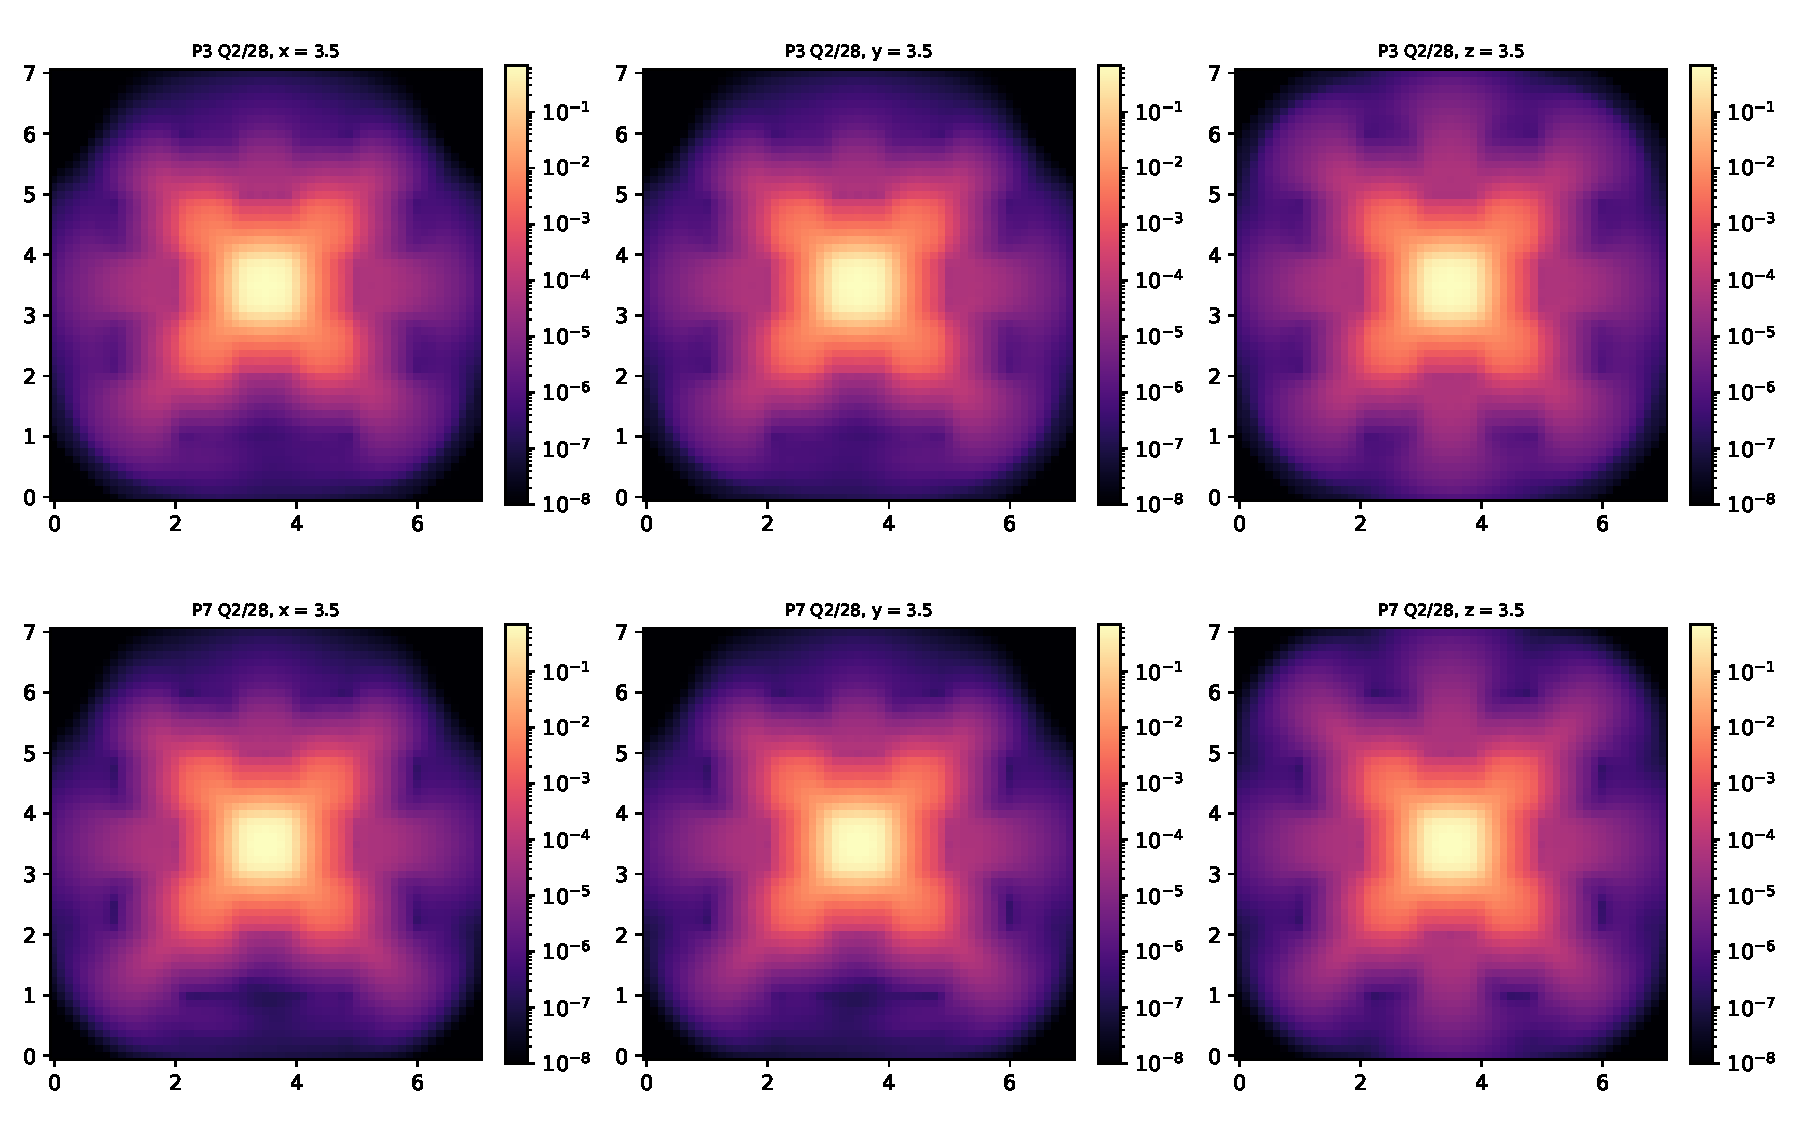
\includegraphics[width=\textwidth]{figures/lattice3d_slices.pdf}
  \caption{3D-Lattice: Dichte in den drei Mittelebenen, feinster Lauf je $P_N$.}
  \label{fig:lattice3d}
\end{figure}

Die Bilanz ist in allen Läufen bis auf $6\cdot10^{-12}$ erfüllt, der M1-Kegel bleibt erhalten. Die
Masse bei $T$ ändert sich zwischen den Auflösungen aber noch um 20 bis 50\,\%
(Tabelle~\ref{tab:lattice3d}); die Lösung ist auf diesen Gittern \emph{nicht} konvergiert. Bei
29 Punkten pro Achse ist der Unterschied zwischen $P_3$ und $P_7$ kleiner als $0.3\,\%$, der
Ortsfehler dominiert also vollständig. Für quantitative Aussagen sind Gitter mit mindestens acht
Zellen pro Materialwürfel nötig. Der Test dient hier als Robustheits- und Bilanztest in drei
Dimensionen.

Die Monte-Carlo-Referenz (wie im 2D-Fall, $4\cdot10^{10}$ Historien) ergibt $M(T)=0.702146$,
$A=2.497854$ und $R(T)=0.993430$ mit statistischen Fehlern um $10^{-5}$. Gegen sie liegt die Masse
für $Q_1$ und $P_7$ auf $56^3$, $112^3$ und $168^3$ Elementen bei $-20.1\,\%$, $-8.9\,\%$ und
$-5.8\,\%$; die Rate bei $T$ liegt durchweg unter $0.4\,\%$. Ab $112^3$ ist auch der
$P_N$-Fehler wesentlich ($168^3$: $P_3$ $-9.0\,\%$, $P_7$ $-5.8\,\%$), sodass sich Orts- und
Winkelfehler auf diesen Gittern nicht sauber trennen lassen. Die First-Collision-Source verkleinert
den Massenfehler bei gleichem Gitter etwa um den Faktor drei ($P_7$: $56^3$ $-7.1\,\%$, $112^3$
$-3.0\,\%$).

\section{Shadow-Test (archiviert)}
\label{sec:tests:shadow}

Der Shadow-Test nach \cite[Abschnitt~4.2.1]{weih_2020} schickt einen kollimierten Strahl durch
das Gebiet $(-0.75,0.75)\times(-0.25,0.25)^2$ auf eine stark absorbierende Kugel ($R=0.1$,
$\sigma_a\in\{1,10,100,10^7\}$). Als Referenz dient die unkollidierte Beer-Lambert-Lösung
\[
  \rho(x,y,z)=\rho_b(y,z)\exp\bigl(-\sigma_a\,\ell(x,y,z)\bigr)
\]
mit der Sehnenlänge $\ell$ des Strahls durch die Kugel. Das Strahlprofil ist in
\cite{weih_2020} nicht angegeben; wir verwenden $\rho_b=1$ für $r\le0.15$ mit
$\cos^2$-Übergang bis $r=0.2$.

Der Test ist für die weitere Validierung archiviert. Gründe:
\begin{itemize}
  \item Schon der freie Strahl wird von $P_N$ mit $N\le11$ nicht wiedergegeben
        (Abbildung~\ref{fig:shadow}). Der Einstrom ist korrekt, aber der $\delta$-Strahl in der
        Richtung zerfließt quer und füllt die schmale Box. Bei $x=0.5$ liegt $\rho$ auf der Achse
        bei $\sigma_a=1$ bei 0.24 ($P_7$) bzw.\ 0.48 ($P_{11}$) statt 0.82. Für
        $\sigma_a\ge100$ füllt sich der Schatten seitlich auf.
  \item Die Abweichung misst damit fast ausschließlich den Winkelmodellfehler, nicht das Verfahren.
  \item \cite{weih_2020} rechnet den Test mit einem Lattice-Boltzmann-Verfahren, dessen Stencil eine
        diskrete Richtung exakt entlang des Strahls enthält; dort ist der Test trivial. Ergebnis ist
        ein einzelnes Farbbild ohne Referenz und ohne Fehlerzahl; $M1$ oder $P_N$ wurden für diesen
        Test nicht gerechnet.
  \item Mit First-Collision-Aufspaltung wäre die Lösung wegen $\sigma_s=0$ rein unkollidiert und
        gleich Beer-Lambert; der Test prüfte dann nur den unkollidierten Löser.
\end{itemize}

\begin{figure}[htbp]
  \centering
  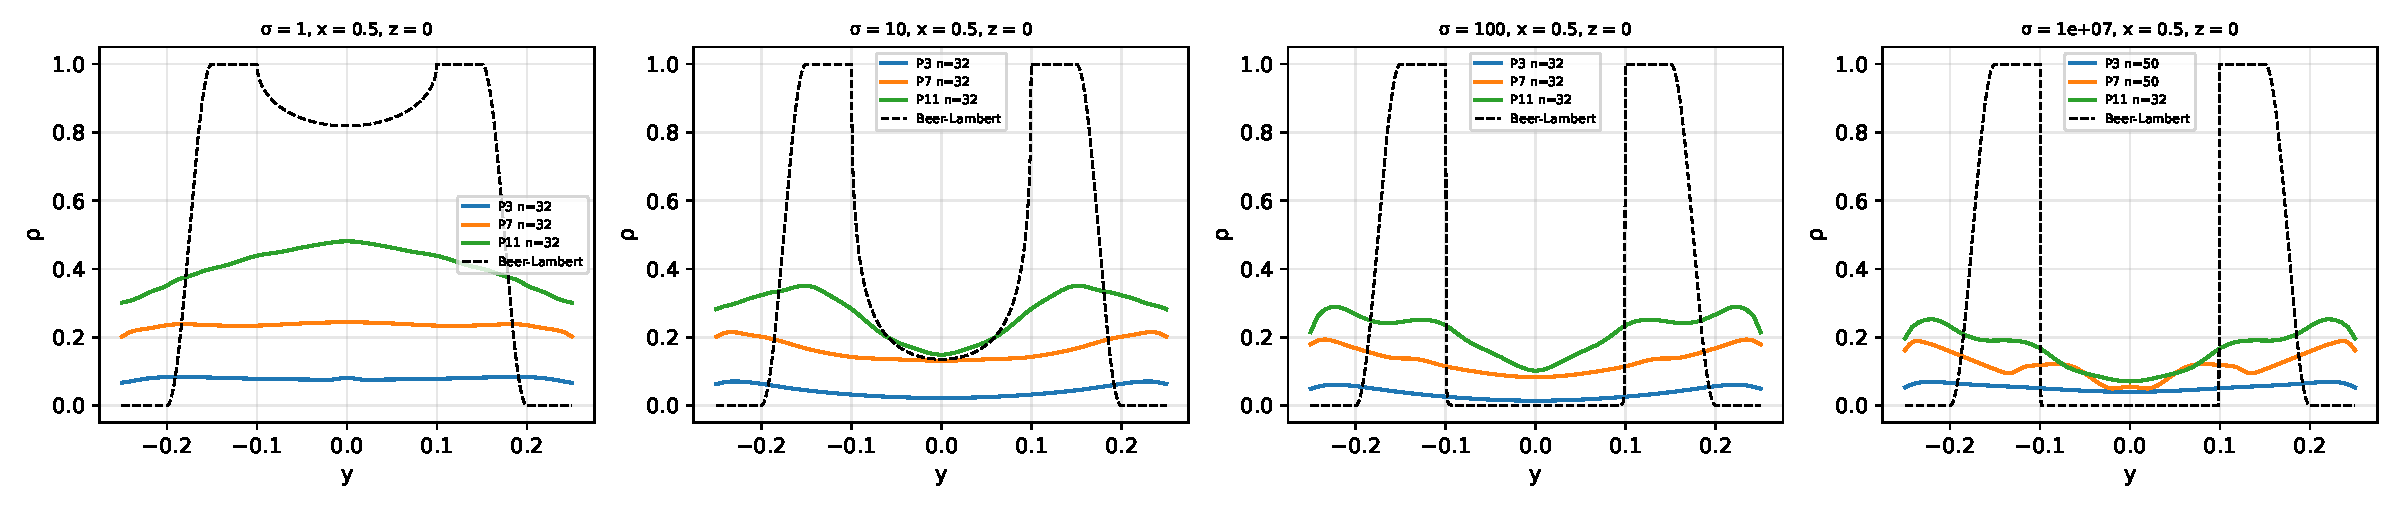
\includegraphics[width=\textwidth]{figures/shadow_profiles.pdf}
  \caption{Shadow-Test (archiviert): Querprofile bei $x=0.5$, $z=0$ für $P_3$, $P_7$, $P_{11}$ auf
           dem feinsten Gitter gegen Beer-Lambert (gestrichelt).}
  \label{fig:shadow}
\end{figure}

Zur Diagnose wurde das $P_N$-Ziel durch ein M1-Galerkin-Ziel mit Levermore-Fluss ersetzt. Bei
$n=8$, $\sigma_a=10$ hält M1 den Strahl zusammen (Dichte am Strahlrand bei $x=0.5$: 0.45 gegen
Referenz 0.5; $P_7$: 0.15) und wirft einen Schatten. Hinter der Kugel ist dieser Schatten zu tief und
schließt sich durch Verschmelzen der Teilstrahlen, die bekannte Schwäche von M1 bei sich kreuzenden
Strahlen.

\section{Robustheit und Rechenaufwand}
\label{sec:tests:robust}

\begin{itemize}
  \item \textbf{Massenbilanz.} In allen Läufen gilt
        \[
          M(T)-M(0)+B+A-S-N_{\mathrm{nudge}}=0
        \]
        bis auf einen relativen Fehler von höchstens $6\cdot10^{-12}$ ($B$: Randausfluss,
        $S$: Quelle, $N_{\mathrm{nudge}}$: gezählte Rundungskorrektur).
  \item \textbf{Realisierbarkeit.} Die Momente niedriger Ordnung liegen nach jedem Schritt im
        M1-Kegel, auch bei $\sigma_a=10^7$. Ein Abbruch bei subnormalen Zuständen
        ($\rho\approx10^{-316}$) wurde durch eine gezählte Aufrundung behoben; die Zusatzmasse liegt
        bei $10^{-317}$.
  \item \textbf{Steife Reaktion.} Absorption bis $\sigma_a=10^7$ braucht keine Sonderbehandlung, weil
        die Reaktion exakt integriert wird.
  \item \textbf{Aufwand.} Gegenüber Pfad~B ist Element-WENO bei gleicher Genauigkeit etwa zwölfmal
        schneller (2D-Lattice, $P_7$, $Q_1/112$). Die Kosten wachsen mit $N$ moderat
        ($Q_1/112$: $P_3\to P_{11}$ Faktor 1.6; $Q_1/224$: $P_7\to P_{11}$ Faktor 1.2).
\end{itemize}

\section{Fazit}
\label{sec:tests:fazit}

Das Verfahren ist robust und effizient: Masse und Realisierbarkeit bleiben in allen Tests bis auf
Rundung erhalten, und gegenüber dem unabhängigen Pfad~B ergibt sich gleiche Genauigkeit bei etwa
einem Zwölftel der Rechenzeit. Im einzigen Test mit kinetischer Referenz für ein heterogenes Medium,
dem 2D-Lattice, konvergieren die Kenngrößen mit dem Gitter; mit $P_{11}$ auf $225^2$ Punkten liegt die
Absorptionsrate $1\,\%$ neben der Referenz, vergleichbar mit auf die Referenz trainierten Surrogaten
\cite{gonzales_2026}.

Die Grenzen liegen im Winkelmodell, nicht in der Diskretisierung: Bei geringer Regularität in der
Richtung (Line Source ohne Filter, kollimierter Strahl im Shadow-Test) bestimmt der
$P_N$-Abbruchfehler das Ergebnis, und Gitterverfeinerung hilft nicht. Hohe Polynomgrade bringen bei
Materialsprüngen keinen Gewinn.

Offen sind:
\begin{itemize}
  \item ein Strahltest mit Streuung und kinetischer Referenz anstelle des Shadow-Tests;
  \item der 1D-Plane-Source-Test gegen die analytische Lösung, für den
        \cite{schneider_leibner_2022} Fehlerkurven verschiedener Momentenmodelle liefert;
  \item der 3D-Lattice auf feineren Gittern (Referenz liegt jetzt vor);
  \item die Wiederholung der Line Source mit dem aktuellen Stand und angepasster Filterstärke für
        $P_{11}$.
\end{itemize}
